\chapter{Duality}
In the last chapter, we explored the Karush-Kuhn-Tucker (KKT) conditions and identified constraints called the \textit{dual feasibility} constraints. In this section, we show that to each linear programming problem (the primal problem) we may associate another linear programming problem (the dual linear programming problem). These two problems are closely related to each other and an analysis of the dual problem can provide deep insight into the primal problem. 


\section{The Dual Problem}
Consider the linear programming problem 
\begin{equation}
P\left\{
\begin{aligned}
\max\;\; & \mathbf{c}^T\mathbf{x}\\
s.t.\;\; & \mathbf{A}\mathbf{x} \leq \mathbf{b}\\
& \mathbf{x} \geq 0
\end{aligned}\right.
\end{equation}

Then the dual problem for Problem $P$ is:
\begin{equation}
D\left\{
\begin{aligned}
\min\;\; & \mathbf{w}\mathbf{b}\\
s.t.\;\; & \mathbf{w}\mathbf{A} \geq \mathbf{c}\\
& \mathbf{w} \geq \mathbf{0}
\end{aligned}\right.
\end{equation}

\begin{remark} Let $\mathbf{v}$ be a vector of \textit{surplus} variables. Then we can transform Problem $D$ into standard form as:
\begin{equation}
D_S\left\{
\begin{aligned}
\min\;\; & \mathbf{w}\mathbf{b}\\
s.t.\;\; & \mathbf{w}\mathbf{A} - \mathbf{v} = \mathbf{c}\\
& \mathbf{w} \geq \mathbf{0}\\
& \mathbf{v} \geq \mathbf{0}
\end{aligned}\right.
\end{equation}
Thus we already see an intimate relationship between duality and the KKT conditions. The feasible region of the dual problem (in standard form) is precisely the the dual feasibility constraints of the KKT conditions for the primal problem.

In this formulation, we see that we have assigned a dual variable $w_i$ ($i=1,\dots,m$) to each constraint in the system of equations $\mathbf{A}\mathbf{x} \leq \mathbf{b}$ of the primal problem. Likewise dual variables $\mathbf{v}$ can be thought of as corresponding to the constraints in $\mathbf{x} \geq \mathbf{0}$. 
\end{remark}

\begin{lemma} The dual of the dual problem is the primal problem.
\label{lem:DualDual}
\end{lemma}
\begin{proof} Rewrite Problem $D$ as:
\begin{equation}
\left\{
\begin{aligned}
\max\;\; & -\mathbf{b}^T\mathbf{w}^T\\
s.t.\;\; & -\mathbf{A}^T\mathbf{w}^T \leq -\mathbf{c}^T\\
& \mathbf{w}^T \geq \mathbf{0}
\end{aligned}\right.
\end{equation}
Let $\boldsymbol{\beta} = -\mathbf{b}^T$, $\mathbf{G} = -\mathbf{A}^T$, $\mathbf{u} = \mathbf{w}^T$ and $\boldsymbol{\kappa} = -\mathbf{c}^T$. Then this new problem becomes:
\begin{equation}
\left\{
\begin{aligned}
\max\;\; & \boldsymbol{\beta}\mathbf{u}\\
s.t.\;\; & \mathbf{G}\mathbf{u} \leq \boldsymbol{\kappa}\\
& \mathbf{u} \geq \mathbf{0}
\end{aligned}\right.
\end{equation}
Let $\mathbf{x}^T$ be the vector of dual variables (transposed) for this problem. We can formulate the dual problem as:
\begin{equation}
\left\{
\begin{aligned}
\min\;\; & \mathbf{x}^T\boldsymbol{\kappa}\\
s.t.\;\; & \mathbf{x}^T\mathbf{G} \geq \boldsymbol{\beta}\\
& \mathbf{x}^T \geq \mathbf{0}
\end{aligned}\right.
\end{equation}
Expanding, this becomes:
\begin{equation}
\left\{
\begin{aligned}
\min\;\; & -\mathbf{x}^T\mathbf{c}^T\\
s.t.\;\; & -\mathbf{x}^T\mathbf{A}^T \geq -\mathbf{b}^T\\
& \mathbf{x}^T \geq \mathbf{0}
\end{aligned}\right.
\end{equation}
This can be simplified to:
\begin{equation}
P\left\{
\begin{aligned}
\max\;\; & \mathbf{c}^T\mathbf{x}\\
s.t.\;\; & \mathbf{A}\mathbf{x} \leq \mathbf{b}\\
& \mathbf{x} \geq 0
\end{aligned}\right.
\end{equation}
as required. This completes the proof.
\end{proof}

Lemma \ref{lem:DualDual} shows that the notion of dual and primal can be exchanged and that it is simply a matter of perspective which problem is the dual problem and which is the primal problem. Likewise, by transforming problems into canonical form, we can develop dual problems for any linear programming problem. 

The process of developing these formulations can be exceptionally tedious, as it requires enumeration of all the possible combinations of various linear and variable constraints. The following table summarizes the process of converting an arbitrary primal problem into its dual. This table can be found in Chapter 6 of \cite{BJS04}.

\begin{table}[hbt]
\centering
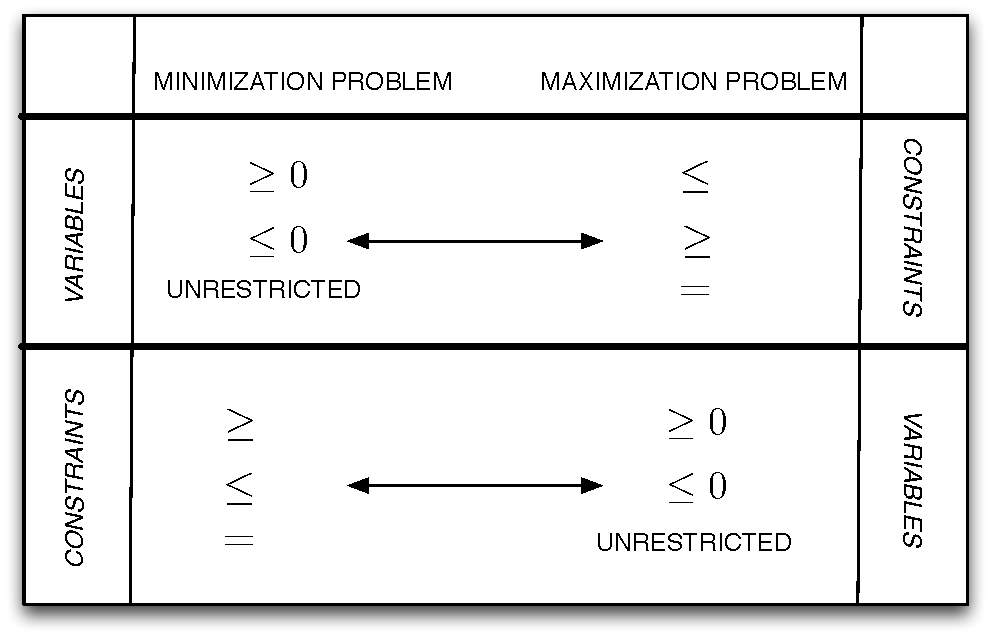
\includegraphics[scale=0.5]{DualConversionTable.pdf}
\caption{Table of Dual Conversions: To create a dual problem, assign a dual variable to each constraint of the form $\mathbf{A}\mathbf{x} \circ \mathbf{b}$, where $\circ$ represents a binary relation. Then use the table to determine the appropriate sign of the inequality in the dual problem as well as the nature of the dual variables.}
\label{tab:Duality}
\end{table}

\begin{example} Consider the problem of finding the dual problem for the Toy Maker Problem (Example \ref{ex:ToyMaker}) in standard form. The primal problem is:
\begin{displaymath}
\begin{aligned}
\max\;\;&7x_1 + 6x_2\\
s.t.\;\;& 3x_1 + x_2 + s_1 = 120\quad & (w_1)\\
& x_1 + 2x_2 + s_2 = 160\quad & (w_2)\\
&x_1 + s_3 = 35\quad & (w_3)\\
&x_1, x_2, s_1, s_2, s_3 \geq 0
\end{aligned}
\end{displaymath}
Here we have placed dual variable names ($w_1$, $w_2$ and $w_3$) next to the constraints to which they correspond. 

The primal problem variables in this case are all positive, so using Table \ref{tab:Duality} we know that the constraints of the dual problem will be greater-than-or-equal-to constraints. Likewise, we know that the dual variables will be unrestricted in sign since the primal problem constraints are all equality constraints.

The coefficient matrix is:
\begin{displaymath}
\mathbf{A} = 
\begin{bmatrix}
3 & 1 & 1 & 0 & 0\\
1 & 2 & 0 & 1 & 0\\
1 & 0 & 0 & 0 & 1
\end{bmatrix}
\end{displaymath}
Clearly we have:
\begin{gather*}
\mathbf{c} = \begin{bmatrix}7 & 6 & 0 & 0 & 0\end{bmatrix}\\
\mathbf{b}= \begin{bmatrix}120 \\160 \\ 35\end{bmatrix}
\end{gather*} 
Since $\mathbf{w} = [w_1 \;\; w_2 \;\; w_3]$, we know that $\mathbf{w}\mathbf{A}$ will be:
\begin{displaymath}
\mathbf{w}\mathbf{A} = 
\begin{bmatrix}
3w_1 + w_2 + w_3 & w_1 + 2w_2 & w_1 & w_2 & w_3
\end{bmatrix}
\end{displaymath}
This vector will be related to $\mathbf{c}$ in the constraints of the dual problem. \textbf{Remember, in this case, all constraints are greater-than-or-equal-to}. Thus we see that the constraints of the dual problem are:
\begin{align*}
3w_1 + w_2 + w_3 \geq 7\\
w_1 + 2w_2 \geq 6\\
w_1 \geq 0\\
w_2 \geq 0\\
w_3 \geq 0 
\end{align*}

We also have the redundant set of constraints that tell us $\mathbf{w}$ is unrestricted because the primal problem had equality constraints. This \textit{will always} happen in cases when  you've introduced slack variables into a problem to put it in standard form. This should be clear from the definition of the dual problem for a maximization problem in canonical form. 

Thus the whole dual problem becomes:
\begin{equation}
\begin{aligned}
\min\;\;&120w_1 + 160w_2 + 35w_3\\
s.t.\;\; & 3w_1 + w_2 + w_3 \geq 7\\
&w_1 + 2w_2 \geq 6\\
&w_1 \geq 0\\
&w_2 \geq 0\\
&w_3 \geq 0 \\
&\mathbf{w}\quad\text{unrestricted}
\end{aligned}
\end{equation}

Again, note that in reality, the constraints we derived from the $\mathbf{w}\mathbf{A}\geq\mathbf{c}$ part of the dual problem make the constraints ``$\mathbf{w}$ unrestricted'' redundant, for in fact $\mathbf{w} \geq \mathbf{0}$ just as we would expect it to be if we'd found the dual of the Toy Maker problem given in canonical form.
\end{example}


\begin{exercise} Identify the dual problem for:
\begin{displaymath}
\begin{aligned}
\max\;\;&x_1 + x_2\\
s.t.\;\;&2x_1 + x_2 \geq 4\\
&x_1 + 2x_2 \leq 6\\
&x_1, x_2 \geq 0
\end{aligned}
\end{displaymath}
\end{exercise}

\begin{exercise} Use the table or the definition of duality to determine the dual for the problem:
\begin{equation}
\left\{
\begin{aligned}
\min\;\; & \mathbf{c}\mathbf{x}\\
s.t.\;\; & \mathbf{A}\mathbf{x} \leq \mathbf{b}\\
& \mathbf{x} \geq 0
\end{aligned}\right.
\end{equation}
Compare it to the KKT conditions you derived in Exercise \ref{exer:MinKKT}.
\end{exercise}

\section{Weak Duality}
There is a deep relationship between the objective function value, feasibility and boundedness of the primal problem and the dual problem. We will explore these relationships in the following lemmas.

\begin{lemma}[Weak Duality] For the primal problem $P$ and dual problem $D$ let $\mathbf{x}$ and $\mathbf{w}$ be feasible solutions to Problem $P$ and Problem $D$ respectively. Then:
\begin{equation}
\mathbf{w}\mathbf{b} \geq \mathbf{c}\mathbf{x}
\label{eqn:WeakDual0}
\end{equation}
\label{lem:WeakDuality}
\end{lemma}
\begin{proof} Primal feasibility ensures that:
\begin{displaymath}
\mathbf{A}\mathbf{x} \leq \mathbf{b}
\end{displaymath}
Therefore, we have:
\begin{equation}
\mathbf{w}\mathbf{A}\mathbf{x} \leq \mathbf{w}\mathbf{b}
\label{eqn:WeakDual1}
\end{equation}

Dual feasibility ensure that:
\begin{displaymath}
\mathbf{w}\mathbf{A} \geq \mathbf{c}
\end{displaymath}
Therefore we have:
\begin{equation}
\mathbf{w}\mathbf{A}\mathbf{x} \geq \mathbf{c}\mathbf{x}
\label{eqn:WeakDual2}
\end{equation}

Combining Equations \ref{eqn:WeakDual1} and \ref{eqn:WeakDual2} yields Equation \ref{eqn:WeakDual0}:
\begin{displaymath}
\mathbf{w}\mathbf{b} \geq \mathbf{c}\mathbf{x}
\end{displaymath}
This completes the proof.
\end{proof}

\begin{remark}
Lemma \ref{lem:WeakDuality} ensures that the optimal solution $\mathbf{w}^*$ for Problem $D$ must provide an \textit{upper bound} to Problem $P$, since for any feasible $\mathbf{x}$, we know that:
\begin{equation}
\mathbf{w}^*\mathbf{b} \geq \mathbf{c}\mathbf{x}
\end{equation}
Likewise, any optimal solution to Problem $P$ provides a lower bound on solution $D$. 
\end{remark}

\begin{corollary} If Problem $P$ is unbounded, then Problem $D$ is infeasible. Likewise, if Problem $D$ is unbounded, then Problem $P$ is infeasible.
\label{cor:WeakDuality2}
\end{corollary} 
\begin{proof} For any $\mathbf{x}$, feasible to Problem $P$ we know  that $\mathbf{w}\mathbf{b} \geq \mathbf{c}\mathbf{x}$ for any feasible $\mathbf{w}$. The fact that Problem $P$ is unbounded implies that for any $V \in \mathbb{R}$ we can find an $\mathbf{x}$ feasible to Problem $P$ that $\mathbf{c}\mathbf{x} > V$. If $\mathbf{w}$ were feasible to Problem $D$, then we would have $\mathbf{w}\mathbf{b} > V$ for any arbitrarily chosen $V$. There can be no finite vector $\mathbf{w}$ with this property and we conclude that Problem $D$ must be infeasible. 

The alternative case that when Problem $D$ is unbounded, then Problem $P$ is infeasible follows by reversing the roles of the problem. This completes the proof.
\end{proof}

\section{Strong Duality}
\begin{lemma} Problem $D$ has an optimal solution $\mathbf{w}^* \in \mathbb{R}^m$ if and only if there exists vector $\mathbf{x}^* \in \mathbb{R}^n$ and $\mathbf{s}^* \in \mathbb{R}^m$ such that:
\begin{align}
\text{Primal Feasibility}&\left\{ 
\begin{aligned}
\mathbf{w}^*\mathbf{A} \geq \mathbf{c}\\
\mathbf{w}^* \geq 0
\label{eqn:KKTDual1}
\end{aligned}\right.\\
\text{Dual Feasibility}&\left\{ 
\begin{aligned}
\mathbf{A}\mathbf{x}^* + \mathbf{s}^* = \mathbf{b}\\
\mathbf{x}^* \geq 0\\
\mathbf{s}^* \geq 0
\label{eqn:KKTDual2}
\end{aligned}\right.\\
\text{Complementary Slackness}&\left\{ 
\begin{aligned}
\left(\mathbf{w}^*\mathbf{A} - \mathbf{c}\right)\mathbf{x}^* = 0\\
\mathbf{w}^*\mathbf{s}^* = 0
\label{eqn:KKTDual3}
\end{aligned}\right.
\end{align}
Furthermore, these KKT conditions are equivalent to the KKT conditions for the primal problem.
\label{lem:DualKKT}
\end{lemma}
\begin{proof} Following the proof of Lemma \ref{lem:DualDual}, let $\boldsymbol{\beta} = -\mathbf{b}^T$, $\mathbf{G} = -\mathbf{A}^T$, $\mathbf{u} = \mathbf{w}^T$ and $\boldsymbol{\kappa} = -\mathbf{c}^T$. Then the dual problem can be rewritten as:
\begin{displaymath}
\left\{
\begin{aligned}
\max\;\; & \boldsymbol{\beta}\mathbf{u}\\
s.t.\;\; & \mathbf{G}\mathbf{u} \leq \boldsymbol{\kappa}\\
& \mathbf{u} \geq \mathbf{0}
\end{aligned}\right.
\end{displaymath}
Let $\mathbf{x}^T \in \mathbb{R}^{1 \times n}$ and $s^T \in \mathbb{R}^{1 \times m}$ be the dual variables for this problem. Then applying Theorem \ref{thm:KKT}, we obtain KKT conditions for this problem:
\begin{align}
\text{Primal Feasibility}&\left\{ 
\begin{aligned}
\mathbf{G}\mathbf{u}^* \leq \boldsymbol{\kappa}\\
\mathbf{u}^* \geq \mathbf{0}
\end{aligned}\right.\\
\text{Dual Feasibility}&\left\{ 
\begin{aligned}
{\mathbf{x}^*}^T\mathbf{G} - {\mathbf{s}^*}^T = \boldsymbol{\beta}\\
{\mathbf{x}^*}^T \geq \mathbf{0}\\
{\mathbf{s}^*}^T \geq \mathbf{0}
\end{aligned}\right.\\
\text{Complementary Slackness}&\left\{ 
\begin{aligned}
{\mathbf{x}^*}^T\left(\mathbf{G}\mathbf{u}^* - \boldsymbol{\kappa}\right) = 0\\
{\mathbf{s}^*}^T\mathbf{u}^* = 0
\end{aligned}\right.
\end{align}
We can rewrite:
\begin{gather*}
\mathbf{G}\mathbf{u}^* \leq \boldsymbol{\kappa} \equiv -\mathbf{A}^T\mathbf{w}^T \leq -\mathbf{c}^T \equiv \mathbf{w}\mathbf{A} \geq \mathbf{c}\\
{\mathbf{x}^*}^T\mathbf{G} - {\mathbf{s}^*}^T = \boldsymbol{\beta} \equiv
{\mathbf{x}^*}^T(-\mathbf{A}^T) - {\mathbf{s}^*}^T = -\mathbf{b}^T \equiv
\mathbf{A}\mathbf{x}^* + \mathbf{s}^* = \mathbf{b}\\
{\mathbf{x}^*}^T\left(\mathbf{G}\mathbf{u}^* - \boldsymbol{\kappa}\right) = 0 \equiv
{\mathbf{x}^*}^T\left((-\mathbf{A}^T){\mathbf{w}^*}^T - (-\mathbf{c}^T)\right) = 0 \equiv (\mathbf{w}^*\mathbf{A} - \mathbf{c})\mathbf{x}^* = 0\\
{\mathbf{s}^*}^T\mathbf{u}^* = 0 \equiv {\mathbf{s}^*}^T{\mathbf{w}^*}^T = 0 \equiv \mathbf{w}^*\mathbf{s}^* = 0
\end{gather*}
Thus, we have shown that the KKT conditions for the dual problem are:
\begin{align*}
\text{Primal Feasibility}&\left\{ 
\begin{aligned}
\mathbf{w}^*\mathbf{A} \geq \mathbf{c}\\
\mathbf{w}^* \geq 0
\end{aligned}\right.\\
\text{Dual Feasibility}&\left\{ 
\begin{aligned}
\mathbf{A}\mathbf{x}^* + \mathbf{s}^* = \mathbf{b}\\
\mathbf{x}^* \geq 0\\
\mathbf{s}^* \geq 0
\end{aligned}\right.\\
\text{Complementary Slackness}&\left\{ 
\begin{aligned}
\left(\mathbf{w}^*\mathbf{A} - \mathbf{c}\right)\mathbf{x}^* = 0\\
\mathbf{w}^*\mathbf{s}^* = 0
\end{aligned}\right.
\end{align*}

To prove the equivalence to the KKT conditions for the primal problem, define:
\begin{gather}
\mathbf{s}^* = \mathbf{b} - \mathbf{A}\mathbf{x}^* \\
\mathbf{v}^* = \mathbf{w}^*\mathbf{A} - \mathbf{c}
\end{gather}
That is, $\mathbf{s}^*$ is a vector slack variables for the primal problem $P$ at optimality and $\mathbf{v}^*$ is a vector of surplus variables for the dual problem $D$ at optimality. Recall the KKT conditions for the primal problem are:
\begin{align*}
\text{Primal Feasibility}&\left\{ 
\begin{aligned}
\mathbf{A}\mathbf{x}^* \leq \mathbf{b}\\
\mathbf{x}^* \geq \mathbf{0}
\end{aligned}\right.\\
\text{Dual Feasibility}&\left\{ 
\begin{aligned}
\mathbf{w}^*\mathbf{A} - \mathbf{v}^* = \mathbf{c}\\
\mathbf{w}^* \geq \mathbf{0}\\
\mathbf{v}^* \geq \mathbf{0}
\end{aligned}\right.\\
\text{Complementary Slackness}&\left\{ 
\begin{aligned}
\mathbf{w}^*\left(\mathbf{A}\mathbf{x}^* - \mathbf{b}\right) = 0\\
\mathbf{v}^*\mathbf{x}^* = 0
\end{aligned}\right.
\end{align*}

We can rewrite these as:
\begin{align}
\text{Primal Feasibility}&\left\{ 
\begin{aligned}
\mathbf{A}\mathbf{x}^* + \mathbf{s}^* = \mathbf{b}\\
\mathbf{x}^* \geq \mathbf{0}
\end{aligned}\right.\\
\text{Dual Feasibility}&\left\{ 
\begin{aligned}
\mathbf{w}^*\mathbf{A} - \mathbf{v}^* = \mathbf{c}\\
\mathbf{w}^* \geq \mathbf{0}\\
\mathbf{v}^* \geq \mathbf{0}
\end{aligned}\right.\\
\text{Complementary Slackness}&\left\{ 
\begin{aligned}
\mathbf{w}^*\left(\mathbf{s}^*\right) = 0\\
\mathbf{v}^*\mathbf{x}^* = 0
\end{aligned}\right.
\end{align}
Where the complementary slackness condition $\mathbf{w}^*(\mathbf{A}\mathbf{x}^* - \mathbf{b}) = 0$ is re-written as:
\begin{displaymath}
\mathbf{w}^*(\mathbf{A}\mathbf{x}^* - \mathbf{b}) = 0 \equiv \mathbf{w}^*(-(\mathbf{b} - \mathbf{A}\mathbf{x}^*) = 0 \equiv \mathbf{w}^*(-\mathbf{s}^*) = 0 \equiv \mathbf{w}^*(\mathbf{s}^*) 
\end{displaymath}

Likewise beginning with the KKT conditions for the dual problem (Expression \ref{eqn:KKTDual1} - \ref{eqn:KKTDual3}) we can write:
\begin{align*}
\text{Primal Feasibility}&\left\{ 
\begin{aligned}
\mathbf{w}^*\mathbf{A} - \mathbf{v}^* \geq \mathbf{c}\\
\mathbf{w}^* \geq 0
\end{aligned}\right.\\
\text{Dual Feasibility}&\left\{ 
\begin{aligned}
\mathbf{A}\mathbf{x}^* + \mathbf{s}^* = \mathbf{b}\\
\mathbf{x}^* \geq 0\\
\mathbf{s}^* \geq 0
\end{aligned}\right.\\
\text{Complementary Slackness}&\left\{ 
\begin{aligned}
\left(\mathbf{v}^*\right)\mathbf{x}^* = 0\\
\mathbf{w}^*\mathbf{s}^* = 0
\end{aligned}\right.
\end{align*}
Here we substitute $\mathbf{v}^*$ for $\mathbf{w}^*\mathbf{A} - \mathbf{c}$ in the complementary slackness terms. Thus we can see that the KKT conditions for the primal and dual problems are equivalent. This completes the proof.
\end{proof}
\begin{remark} Notice that the KKT conditions for the primal and dual problems are equivalent, but the dual feasibility conditions for the primal problem are identical to the primal feasibility conditions for the dual problem and vice-versa. Thus, two linear programming problems are dual to each other if they share KKT conditions with the primal and dual feasibility conditions swapped.
\end{remark}


\begin{exercise} Compute the dual problem for a canonical form minimization problem:
\begin{displaymath}
P\left\{
\begin{aligned}
\min\;\;&\mathbf{c}\mathbf{x}\\
s.t.\;\;&\mathbf{A}\mathbf{x} \geq \mathbf{b}\\
& \mathbf{x} \geq \mathbf{0}
\end{aligned}\right.
\end{displaymath}
Find the KKT conditions for the dual problem you just identified. Use the result from Exercise \ref{exer:MinKKT} to show that KKT conditions for Problem $P$ are identical to the KKT conditions for the dual problem you just found.
\end{exercise}
%\begin{exercise} Prove Lemma \ref{lem:DualKKT}. [Hint: Transform Problem $D$ into a canonical form maximization problem and find the KKT conditions where the dual variables are $\mathbf{x}^*$ and $\mathbf{s}^*$. Then simplify the KKT conditions to obtain those stated in the formula. To prove equivalence, let $\mathbf{v} = \mathbf{w}\mathbf{A} - \mathbf{c}$ with $\mathbf{v} \geq \mathbf{0}$. Argue that $\mathbf{A}\mathbf{x}^* + \mathbf{s}^* = \mathbf{b}$, $\mathbf{x}^*,\mathbf{s}^* \geq \mathbf{0}$ implies that $\mathbf{x}^*$ is feasible to the primal problem. Then show that by subtituting in $\mathbf{v}^*$ for $\mathbf{w}^*\mathbf{A} - \mathbf{c}$ and $\mathbf{s}^* = \mathbf{b}-\mathbf{A}\mathbf{x}^*$ that the complementary slackness conditions for both problems are identical.]
%\end{exercise}

\begin{lemma}[Strong Duality] There is a bounded optimal solution $\mathbf{x}^*$ for Problem $P$ if and only if there is a bounded optimal solution $\mathbf{w}^*$ for Problem $D$. Furthermore, $\mathbf{c}\mathbf{x}^* = \mathbf{w}^*\mathbf{b}$.
\label{lem:StrongDuality}
\end{lemma}
\begin{proof} Suppose that there is a solution $\mathbf{x}^*$ for Problem $P$. Let $\mathbf{s}^* = \mathbf{b} - \mathbf{A}\mathbf{x}^*$. Clearly $\mathbf{s}^* \geq \mathbf{0}$. 

By Theorem \ref{thm:KKT} there exists dual variables $\mathbf{w}^*$ and $\mathbf{v}^*$ satisfying dual feasibility and complementary slackness. Dual feasibility in the KKT conditions implies that:
\begin{equation}
\mathbf{v}^* = \mathbf{w}^*\mathbf{A} - \mathbf{c}
\end{equation}
We also know that $\mathbf{w}^*,\mathbf{v}^* \geq \mathbf{0}$. Complementary Slackness (from Theorem \ref{thm:KKT}) states that $\mathbf{v}^*\mathbf{x}^* = 0$. But $\mathbf{v}^*$ is defined above and we see that: 
\begin{equation}
\mathbf{v}^*\mathbf{x}^* = 0 \implies \left(\mathbf{w}^*\mathbf{A} - \mathbf{c}\right)\mathbf{x} = 0
\end{equation}

Likewise, since we have $\mathbf{s}^* = \mathbf{b} - \mathbf{A}\mathbf{x}^*$. Complementary slackness assures us that $\mathbf{w}^*\left(\mathbf{b} - \mathbf{A}\mathbf{x}^*\right) = 0$. Thus we see that:
\begin{equation}
\mathbf{w}^*\left(\mathbf{b} - \mathbf{A}\mathbf{x}^*\right) = 0 \implies \mathbf{w}^*\mathbf{s}^* = 0
\end{equation}
Thus it follows from Lemma  \ref{lem:DualKKT} that $\mathbf{w}^*$ is an optimal solution to Problem $D$ since it satisfies the KKT conditions. The fact that Problem $P$ has an optimal solution when Problem $D$ has an optimal solution can be proved in a similar manner starting with the KKT conditions given in Lemma \ref{lem:DualKKT} and applying the same reasoning as above. 

Finally, at optimality, we know from Lemma \ref{lem:DualKKT} that:
\begin{equation}
\left(\mathbf{w}^*\mathbf{A} - \mathbf{c}\right)\mathbf{x}^* = 0 \implies \mathbf{w}^*\mathbf{A}\mathbf{x}^* = \mathbf{c}\mathbf{x}^*
\end{equation}
We also know from Theorem \ref{thm:KKT} that:
\begin{equation}
\mathbf{w}^*\left(\mathbf{b} - \mathbf{A}\mathbf{x}^*\right) = 0\implies  \mathbf{w}^*\mathbf{b} = \mathbf{w}^*\mathbf{A}\mathbf{x}^*
\end{equation}
Therefore we have: $\mathbf{w}^*\mathbf{b} = \mathbf{c}\mathbf{x}^*$. This completes the proof.
\end{proof}

\begin{corollary} If Problem $P$ is infeasible, then Problem $D$ is either unbounded or infeasible. If Problem $D$ is infeasible, then either Problem $P$ is unbounded or infeasible.
\label{cor:DualInfeas}
\end{corollary}
\begin{proof} This result follows by contrapositive from Lemma \ref{lem:StrongDuality}. To see this, suppose that Problem $P$ is infeasible. Then Problem $P$ has no bounded optimal solution. Therefore, Problem $D$ has no bounded optimal solution (by Lemma \ref{lem:StrongDuality}). If Problem $D$ has no bounded optimal solution, then either Problem $D$ is unbounded or it is infeasible. A symmetric argument on Problem $D$ completes the proof of the Lemma. 
\end{proof}

\begin{exercise} Consider the problem 
\begin{displaymath}
\begin{aligned}
\max\;\;&x_1 + x_2\\
s.t.\;\;&x_1 - x_2 \geq 1\\
& -x_1 + x_2 \geq 1\\
&x_1,x_2 \geq 0
\end{aligned}
\end{displaymath}
\begin{enumerate}
\item Show that this problem is infeasible. 
\item Compute its dual. 
\item Show that the dual is infeasible, thus illustrating Corollary \ref{cor:DualInfeas}.
\end{enumerate}
\end{exercise}

The following theorem summarizes all of the results we have obtained in the last two sections.
\begin{theorem}[Strong Duality Theorem] Consider Problem $P$ and Problem $D$. Then exactly one of the following statements is true:
\begin{enumerate*}
\item Both Problem $P$ and Problem $D$ possess optimal solutions $\mathbf{x}^*$ and $\mathbf{w}^*$ respectively and $\mathbf{c}\mathbf{x}^* = \mathbf{w}^*\mathbf{b}$.
\item Problem $P$ is unbounded and Problem $D$ is infeasible.
\item Problem $D$ is unbounded and Problem $P$ is infeasible.
\item Both problems are infeasible.
\end{enumerate*}
\label{thm:StrongDuality}
\end{theorem}

\section{Geometry of the Dual Problem}
The geometry of the dual problem is, in essence, exactly the same the geometry of the primal problem insofar as they are both linear programming problems and thus their feasible regions are polyhedral sets\footnote{Thanks for Michael Cline for suggesting this section.}. Certain examples have a very nice geometric visualization. Consider the problem:
\begin{equation}
\left\{
\begin{aligned}
\max\;\; & 6x_1 + 6x_2 \\
s.t.\;\; & 3x_1 + 2x_2 \leq 6\\
 & 2x_1 + 3x_2 \leq 6\\
 & x_1, x_2 \geq 0
\end{aligned}\right.
\label{eqn:SymmetricDual}
\end{equation}
In this problem we have:
\begin{displaymath}
\mathbf{A} = \begin{bmatrix}3 & 2\\2 & 3\end{bmatrix}\quad \mathbf{c} = \begin{bmatrix}6 & 6\end{bmatrix} \quad \mathbf{b} = \begin{bmatrix}6\\6\end{bmatrix}
\end{displaymath}
Notice that $\mathbf{A}$ is a symmetric matrix and $\mathbf{c}^T = \mathbf{b}$ and the dual problem is:
\begin{equation}
\left\{
\begin{aligned}
\min \;\; & 6w_1 + 6w_2 \\
s.t.\;\; & 3w_1 + 2w_2 \geq 6\\
 & 2w_1 + 3w_2 \leq 6\\
 & w_1, w_2 \geq 0
\end{aligned}\right.
\label{eqn:SymmetricDual}
\end{equation}
This results in a geometry in which the dual feasible region is a reflection of the primal feasible region (ignoring non-negativity constraints). This is illustrated in Figure \ref{fig:PrimalDualFeasibleRegion-1}.
\begin{figure}[htbp]
\centering
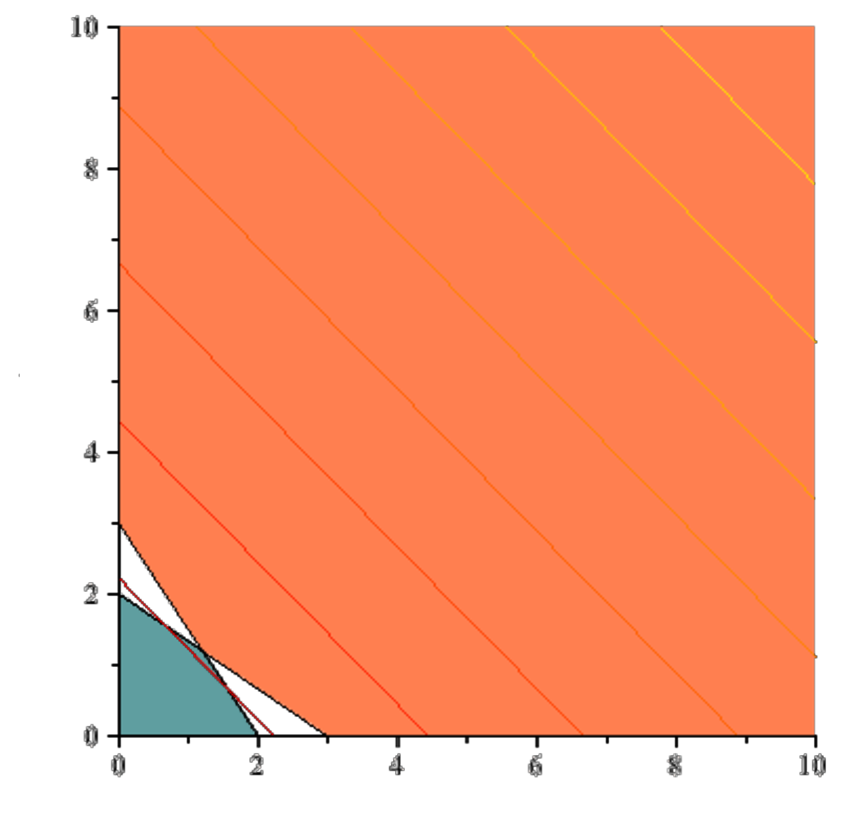
\includegraphics[scale=0.5]{PrimalDualFeasibleRegion-1.pdf}
\caption{The dual feasible region in this problem is a mirror image (almost) of the primal feasible region. This occurs when the right-hand-side vector $\mathbf{b}$ is equal to the objective function coefficient column vector $\mathbf{c}^T$ and the matrix $\mathbf{A}$ is symmetric.}
\label{fig:PrimalDualFeasibleRegion-1} 
\end{figure}

We can also illustrate the process of solving this problem using the (revised) simplex algorithm. In doing so, we first convert Problem \ref{eqn:SymmetricDual} to standard form:
\begin{equation}
\left\{
\begin{aligned}
\max\;\; & 6x_1 + 6x_2 \\
s.t.\;\; & 3x_1 + 2x_2 + s_1 \phantom{+s_2}= 6\\
 & 2x_1 + 3x_2 \phantom{+s_1} + s_2 = 6\\
 & x_1, x_2 \geq 0
\end{aligned}\right.
\label{eqn:SymmetricDual}
\end{equation}
This yields an initial tableau:
\begin{equation}
\begin{array}{c}
z\\
s_1\\
s_2
\end{array}
\left[
\begin{array}{cc|c}
0	&	0	&	0\\
\hline
1	&	0	&   6\\
0	&	1	&	6
\end{array}
\right]
\end{equation}
This is because our initial $\mathbf{c}_\mathbf{B} = \begin{bmatrix}0&0\end{bmatrix}$ and thus $\mathbf{w} = \begin{bmatrix}0&0\end{bmatrix}$. This means at the start of the simplex algorithm, $w_1 = 0$ and $w_2 = 0$ and $x_1 = 0$ and $x_2 = 0$, so we begin at the origin, which is \textbf{in the primal feasible region} and \textbf{not in the dual feasible region}. If we iterate and choose $x_1$ as an entering variable, our updated tableau will be:
\begin{equation}
\begin{array}{c}
z\\
x_1\\
s_2
\end{array}
\left[
\begin{array}{cc|c}
2	&	0	&	12\\
\hline
1/3	&	0	&   2\\
-2/3	&	1	&	2
\end{array}
\right]
\end{equation}
Notice at this point, $x_1 = 2$, $x_2 = 0$ and $w_1 = 2$ and $w_2 = 0$. This point is again feasible for the primal problem but still infeasible for the dual. This step is illustrated in Figure \ref{fig:PrimalDualFeasibleRegion-2}. Entering $x_2$ yields the final tableau:
\begin{equation}
\begin{array}{c}
z\\
x_1\\
x_2
\end{array}
\left[
\begin{array}{cc|c}
6/5	&	6/5	&	72/5\\
\hline
3/5	&	-2/5	&   6/5\\
-2/5	&	3/5	&	6/5
\end{array}
\right]
\end{equation}
At this final point, $x_1 = x_2 = w_1 = w_2 = \tfrac{6}{5}$, which is feasible to both problems. This step is also illustrated in Figure \ref{fig:PrimalDualFeasibleRegion-2}.
\begin{figure}[htbp]
\centering
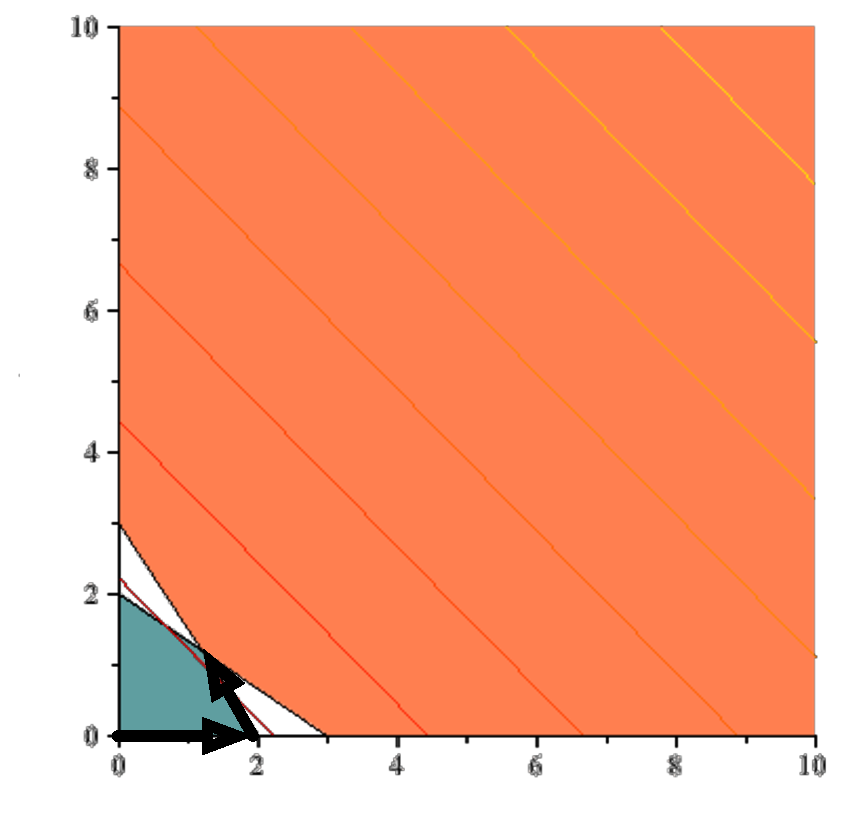
\includegraphics[scale=0.5]{PrimalDualFeasibleRegion-2.pdf}
\caption{The simplex algorithm begins at a feasible point in the feasible region of the primal problem. In this case, this is also the same starting point in the dual problem, which is infeasible. The simplex algorithm moves through the feasible region of the primal problem towards a point in the dual feasible region. At the conclusion of the algorithm, the algorithm reaches the unique point that is both primal and dual feasible.}
\label{fig:PrimalDualFeasibleRegion-2} 
\end{figure}
We should note that this problem is atypical in that the primal and dual feasible regions share one common point. In more standard problems, the two feasible regions cannot be drawn in this convenient way, \textit{but} the simplex process is the same. The simplex algorithm begins at a point in the primal feasible region with a corresponding dual vector that is \textit{not} in the feasible region of the dual problem. As the simplex algorithm progresses, this dual vector approaches and finally enters the dual feasible region.

\begin{exercise} Draw the dual feasible region for the following problem.
\begin{displaymath}
\begin{aligned}
\max\;\; & 3x_1 + 5x_2\\
s.t.\;\; & x_1 + 2x_2 \leq 60\\
& x_1 + x_2 \leq 40\\
& x_1, x_2 \geq 0
\end{aligned}
\end{displaymath}
Solve the problem using the revised simplex algorithm and trace the path of dual variables (the $\mathbf{w}$ vector) in your plot of the dual feasible region. Also trace the path of the primal vector $\mathbf{x}$ through the primal feasible region. [Hint: Be sure to draw the area around the dual feasible region. Your dual vector $\mathbf{w}$ will not enter the feasible region until the last simplex pivot.]
\end{exercise}

\section{Economic Interpretation of the Dual Problem}
Consider again, the value of the objective function in terms of the values of the non-basic variables (Equation \ref{eqn:Obj2}):
\begin{equation}
z=\mathbf{c}\mathbf{x} = 
\mathbf{c_B}\mathbf{B}^{-1}\mathbf{b} + 
\left(\mathbf{c_N} - \mathbf{c_B}\mathbf{B}^{-1}\mathbf{N}\right)\mathbf{x}_N
\end{equation}
Suppose we are at a non-degenerate optimal point. We've already observed that:
\begin{equation}
\frac{\partial z}{\partial x_j} = -(z_j - c_j) = c_j - \mathbf{c}_\mathbf{B}\mathbf{B}^{-1}\mathbf{A}_{\cdot j}
\end{equation}
We can rewrite all these equations in terms of our newly defined term:
\begin{equation}
\mathbf{w} = \mathbf{c}_{\mathbf{B}}\mathbf{B}^{-1}
\end{equation}
to obtain:
\begin{equation}
z = \mathbf{w}\mathbf{b} + 
\left(\mathbf{c_N} - \mathbf{w}\mathbf{N}\right)\mathbf{x}_N
\end{equation}
Remember, $\mathbf{w}$ is the vector of dual variables corresponding to the constraints in our original problem $P$.
 
Suppose we fix the values of $\mathbf{x}_{\mathbf{N}}$. Then we can see that the vector $\mathbf{w}$ has individual elements with the property that:
\begin{equation}
\frac{\partial z}{\partial b_i} = w_i 
\end{equation}
That is, the $i^\text{th}$ element of $\mathbf{w}$ represents the amount that the objective function value would change at optimality assuming we could modify the right-hand-side of the constraints. \textbf{Note, this result holds only in the absence of degeneracy, for reasons we will see in an example.}

Thus, we can think of $w_i$ as the \textit{shadow price} for resource $i$ (the right-hand-side of the $i^\text{th}$ constraint). A shadow price is the \textit{fair price} one would pay for an extra unit of resource $i$. 
\begin{example}
Consider a leather company that requires 1 square yard of leather to make a regular belt and a 1 square yard of leather to make a deluxe belt. If the leather company can use up to 40 square yards per week to construct belts, then one constraint it may have is:
\begin{displaymath}
x_1 + x_2 \leq 40
\end{displaymath}
In the absence of degeneracy, the dual variable (say $w_1$) will tell the fair price we would pay for 1 extra yard of leather. Naturally, if this were not a binding constraint, then $w_1 = 0$ indicating that extra leather is worth \textit{nothing} to us since we already have a surplus of leather.
\end{example} 

To understand the economics of the situation, suppose that we a manufacturer is to produce products $1, \dots, n$ and we produce $x_1,\dots,x_n$ of each. If we can sell each product for a profit of $c_1,\dots,c_n$, then we wish to find values for $x_1,\dots,x_n$ to solve:
\begin{equation}
\max\;\;\sum_{j=1}^{n}c_j x_j
\end{equation}
Simultaneously, suppose that $m$ resources (leather, wood, time etc.) are used to make these $n$ products and that $a_{ij}$ units of resource $i$ are used to manufacture product $j$. Then clearly our constraints will be:
\begin{equation}
a_{i1}x_1 + \dots + a_{in}x_n \leq b_i
\end{equation}
where $b_i$ is the amount of resource $i$ available to the company. Suppose now that the company decides to sell off some of its resources (instead of manufacturing products). Suppose we sell each resource for a price $w_i$ ($i=1,\dots,m$) we'd like to know what a fair price for these resources would be. Each unit of product $j$ not manufactured would result in a \textit{loss of profit} of $c_j$. At the same time, we would obtain a gain (from selling the excess resources) of:
\begin{equation}
\sum_{i=1}^m a_{ij}w_i
\end{equation}
Because we would save $a_{ij}$ units of unit $i$ from \textit{not} manufacturing 1 unit of $x_j$ ($i=1,\dots,m$). Selling this resource would require us to make more money in the sale of the resource then we could in manufacturing the product, or:
\begin{equation}
\sum_{i=1}^m a_{ij}w_i \geq c_j
\end{equation} 
If a selfish profit maximizer wishes to buy these items, then we will seek a price per resource that minimizes the total he could pay for all the items, that is:
\begin{equation}
\min\;\;\sum_{i=1}^{m} w_ib_i
\end{equation}
The Strong Duality Theorem asserts that the optimal solution to this problem will produce \textit{fair shadow prices} that force the total amount an individual could purchase the resources of the company for to be equal to the amount the company could make in manufacturing products itself.

\begin{example}
Assume that a leather company manufactures two types of belts: regular and deluxe. Each belt requires 1 square yard of leather. A regular belt requires 1 hour of skilled labor to produce, while a deluxe belt requires 2 hours of labor. The leather company receives 40 square yards of leather each week and a total of 60 hours of skilled labor is available. Each regular belt nets \$3 in profit, while each deluxe belt nets \$5 in profit. The company wishes to maximize profit. We can compute the fair price the company could sell its time or labor (or the amount the company should be willing to pay to obtain more leather or more hours).

The problem for the leather manufacturer is to solve the linear programming problem:
\begin{displaymath}
\begin{aligned}
\max\;\; & 3x_1 + 5x_2\\
s.t.\;\; & x_1 + 2x_2 \leq 60\\
& x_1 + x_2 \leq 40\\
& x_1, x_2 \geq 0
\end{aligned}
\end{displaymath}

The dual problem for this problem is given as:
\begin{displaymath}
\begin{aligned}
\max\;\; & 60w_1 + 40w_2\\
s.t.\;\; & w_1 + w_2 \geq 3\\
& 2w_1 + w_2 \geq 5\\
& w_1, w_2 \geq 0
\end{aligned}
\end{displaymath}

If we solve the primal problem, we obtain the final revised simplex tableau as:
\begin{displaymath}
\begin{array}{c}
z\\
x_1\\
x_2
\end{array}
\left[
\begin{array}{cc|c}
2	&	1	&	160\\
\hline
-1	&	2	&	20\\
1	&	-1	&	20
\end{array}
\right]
\end{displaymath}
Note that both $x_1$ and $x_2$ are in the basis. In this case, we have $w_1 = 2$ and $w_2 = 1$ from Row 0 of the tableau.

We can likewise solve the dual-problem by converting it to standard form and then using the simplex algorithm, we would have:
\begin{displaymath}
\begin{aligned}
\max\;\; & 60w_1 + 40w_2\\
s.t.\;\; & w_1 + w_2 -v_1 = 3\\
& 2w_1 + w_2 - v_2 = 5\\
& w_1, w_2,v_1,v_2 \geq 0
\end{aligned}
\end{displaymath}
\end{example}
In this case, it is more difficult to solve the dual problem because there is no conveniently obvious initial basic feasible solution (that is, the identity matrix is not embedded inside the coefficient matrix). 

The final full simplex tableau for the dual problem would look like:
\begin{displaymath}
\begin{array}{c}
\\
z\\w_1\\w_2
\end{array}
\left[\begin{array}{c|cccc|c}
z & 	w_1 &	w_2 & 	v_1 &	v_2 & 	RHS\\
\hline
1 & 	0 & 	0 & 	-20 & 	-20 & 	160\\
\hline
0 &  	1 & 	0 & 	1 & 	-1 & 	2\\
0 & 	0 & 	1 & 	-2 & 	1 & 	1
\end{array}\right]
\end{displaymath}

We notice two things: The reduced costs of $v_1$ and $v_2$ are precisely the negatives of the values of $x_1$ and $x_2$. This was to be expected, these variables are duals of each other. However, in a minimization problem, the reduced costs have opposite sign. The second thing to notice is that $w_1 = 2$ and $w_2 = 1$. These are the same values we determined in the primal simplex tableau.

Lastly, let's see what happens if we increase the amount of leather available by 1 square yard. If $w_2$ (the dual variable that corresponds to the leather constraint) is truly a shadow price, then we should predict our profit will increase by 1 unit. Our new problem will become:
\begin{displaymath}
\begin{aligned}
\max\;\; & 3x_1 + 5x_2\\
s.t.\;\; & x_1 + 2x_2 \leq 60\\
& x_1 + x_2 \leq 41\\
& x_1, x_2 \geq 0
\end{aligned}
\end{displaymath}

At optimality, our new revised simplex tableau will be:
\begin{displaymath}
\begin{array}{c}
z\\
x_1\\
x_2
\end{array}
\left[
\begin{array}{cc|c}
2	&	1	&	161\\
\hline
-1	&	2	&	22\\
1	&	-1	&	19
\end{array}
\right]
\end{displaymath}
Thus, if our Leather Manufacturer could obtain leather for a price \textit{under} \$1 per yard. He would be a fool not buy it. Because he could make an immediate profit. This is what economists call \textit{thinking at the margin}. 

\subsection*{Shadow Prices Under Degeneracy}
We have asserted that the value of the dual variable does not necessarily provide a shadow price at a degenerate constraint. To see this, consider the example of the degenerate toy maker problem.
\begin{example}
\begin{displaymath}
\begin{aligned}
\max\;\;&7x_1 + 6x_2\\
s.t.\;\;&3x_1 + x_2 +s_1 = 120\\
&x_1 + 2x_2 + s_2 = 160\\
&x_1 + s_3 = 35\\
&\frac{7}{4}x_1+x_2 + s_4 = 100\\
&x_1,x_2,s_1,s_2,s_3,s_4 \geq 0
\end{aligned}
\end{displaymath}
Recall the optimal full tableau for this problem was:
\begin{displaymath}
\begin{array}{c}
\\
z\\
x_1\\
x_2\\
s_2\\
s_3
\end{array}
\left[
\begin{array}{c|cccccc|c}
z& x_1 & x_2 & s_1 & s_2 & s_3 & s_4 &\text{RHS}\\
\hline
1 & 0 & 0 & 0 & 7/5 	& 0 & 16/5 & 544\\
\hline
0 & 1 & 0 & 0 & -2/5 		& 0  & 4/5 		& 16\\
0 & 0 & 1 & 0 & 7/10 		& 0  & -2/5 	& 72\\
0 & 0 & 0 & 1 & 1/2 		& 0  & -2 		& 0\\
0 & 0 & 0 & 0 & 2/5 		& 1  & -4/5 	& 19
\end{array}\right]
\end{displaymath}
We can compute the dual variables $\mathbf{w}$ for this by using $\mathbf{c}_\mathbf{B}$ and $\mathbf{B}^{-1}$ at optimality. You'll notice that $\mathbf{B}^{-1}$ can always be found in the columns of the slack variables for this problem because we would have begun the simplex algorithm with an identity matrix in that position. We also know that $\mathbf{c}_\mathbf{B} = [7\;\;6\;\;0\;\;0]$ at optimality. Therefore, we can compute $\mathbf{c}_\mathbf{B}\mathbf{B}^{-1}$ as:
\begin{displaymath}
\mathbf{c}_\mathbf{B}\mathbf{B}^{-1} = 
\begin{bmatrix}7&6&0&0\end{bmatrix}
\begin{bmatrix}
 0 & 0 & -2/5 		& 0  & 4/5\\
 1 & 0 & 7/10 		& 0  & -2/5\\
 0 & 1 & 1/2 		& 0  & -2\\
 0 & 0 & 2/5 		& 1  & -4/5
\end{bmatrix} = \begin{bmatrix}0 & 7/5 & 0 & 16/5
\end{bmatrix}
\end{displaymath}
In this case, it would seem that modifying the right-hand-side of constraint 1 would have no affect. This is true, if we were to \textit{increase} the value by a increment of 1. Suppose however we decreased the value of the right-hand-side by 1. Since we claim that:
\begin{equation}
\frac{\partial z}{\partial b_1} = w_1
\end{equation}
there should be no change to the optimal objective function value. However, our new optimal point would occur at $x_1 = 15.6$ and $x_2 = 72.2$ with an objective function value of $542.4$, clearly the value of the dual variable for constraint 1 is not a true representation the shadow price of resource 1. This is illustrated in Figure \ref{fig:DegenDual} where we can see that modifying the right-hand-side of Constraint 1 is transforming the feasible region in a way that substantially changes the optimal solution. This is simply not detected because degeneracy in the primal problem leads to alternative optimal solutions in the dual problem. 

\begin{figure}[htbp]
\subfigure[Original Problem]{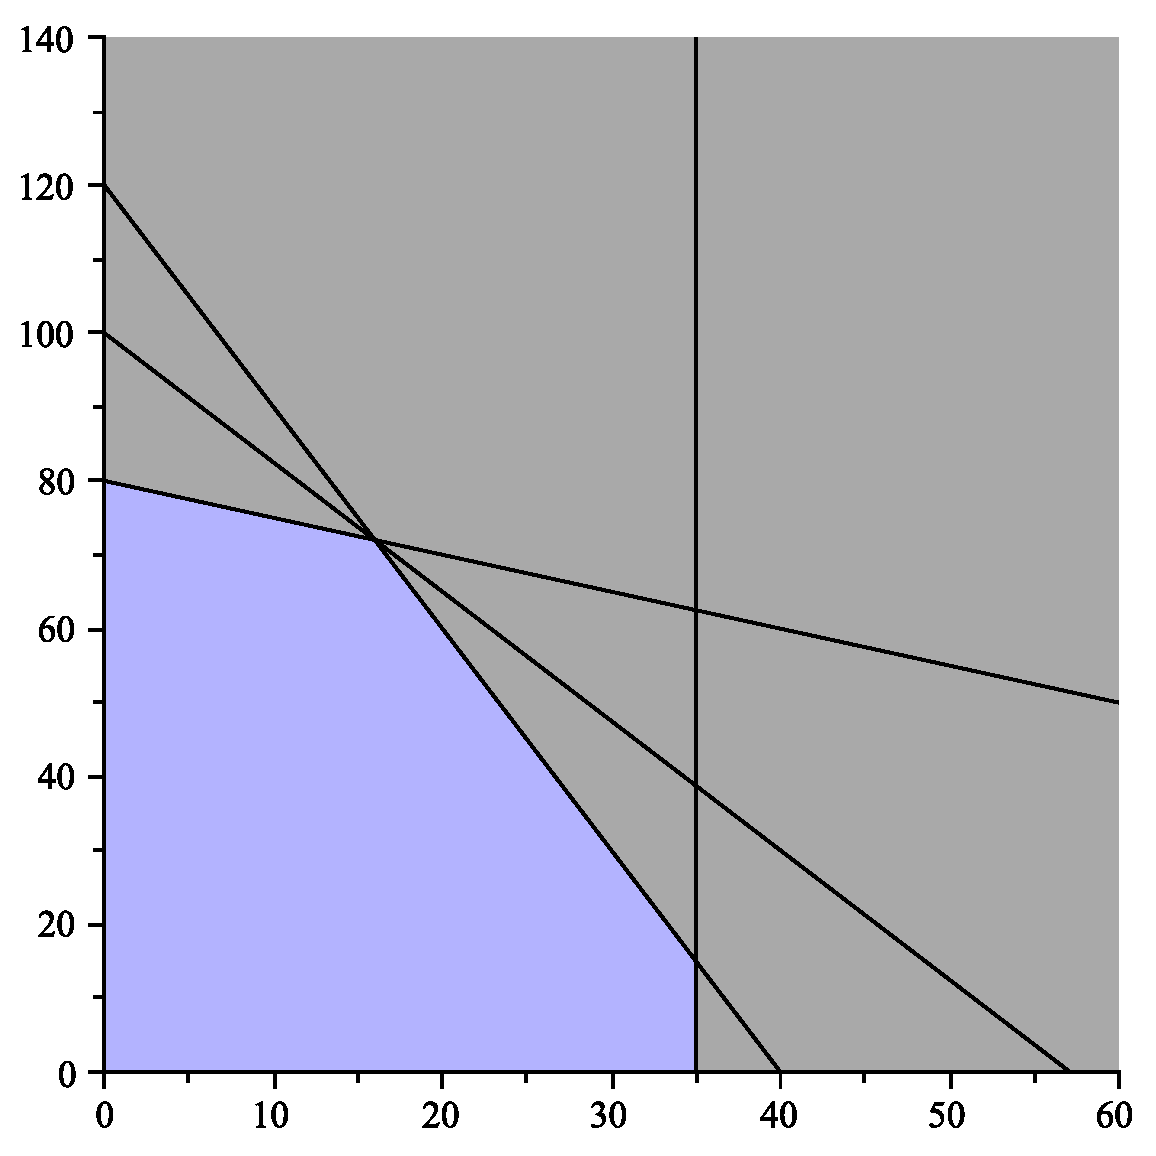
\includegraphics[scale=0.25]{DualDegeneracy1.pdf}}
\subfigure[RHS Decreased]{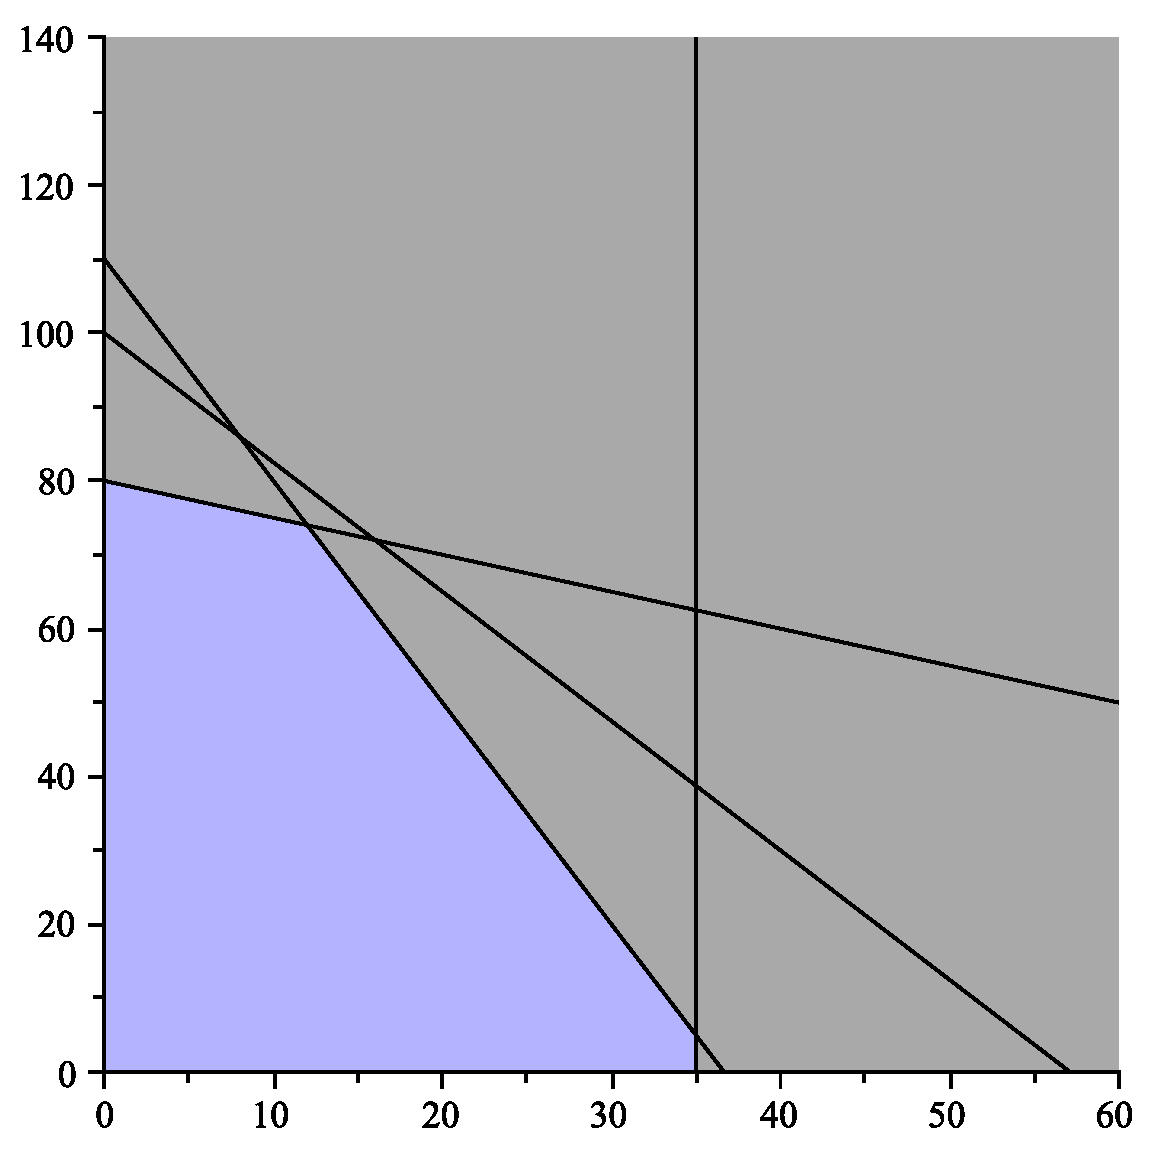
\includegraphics[scale=0.25]{DualDegeneracy2.pdf}}
\subfigure[RHS Increased]{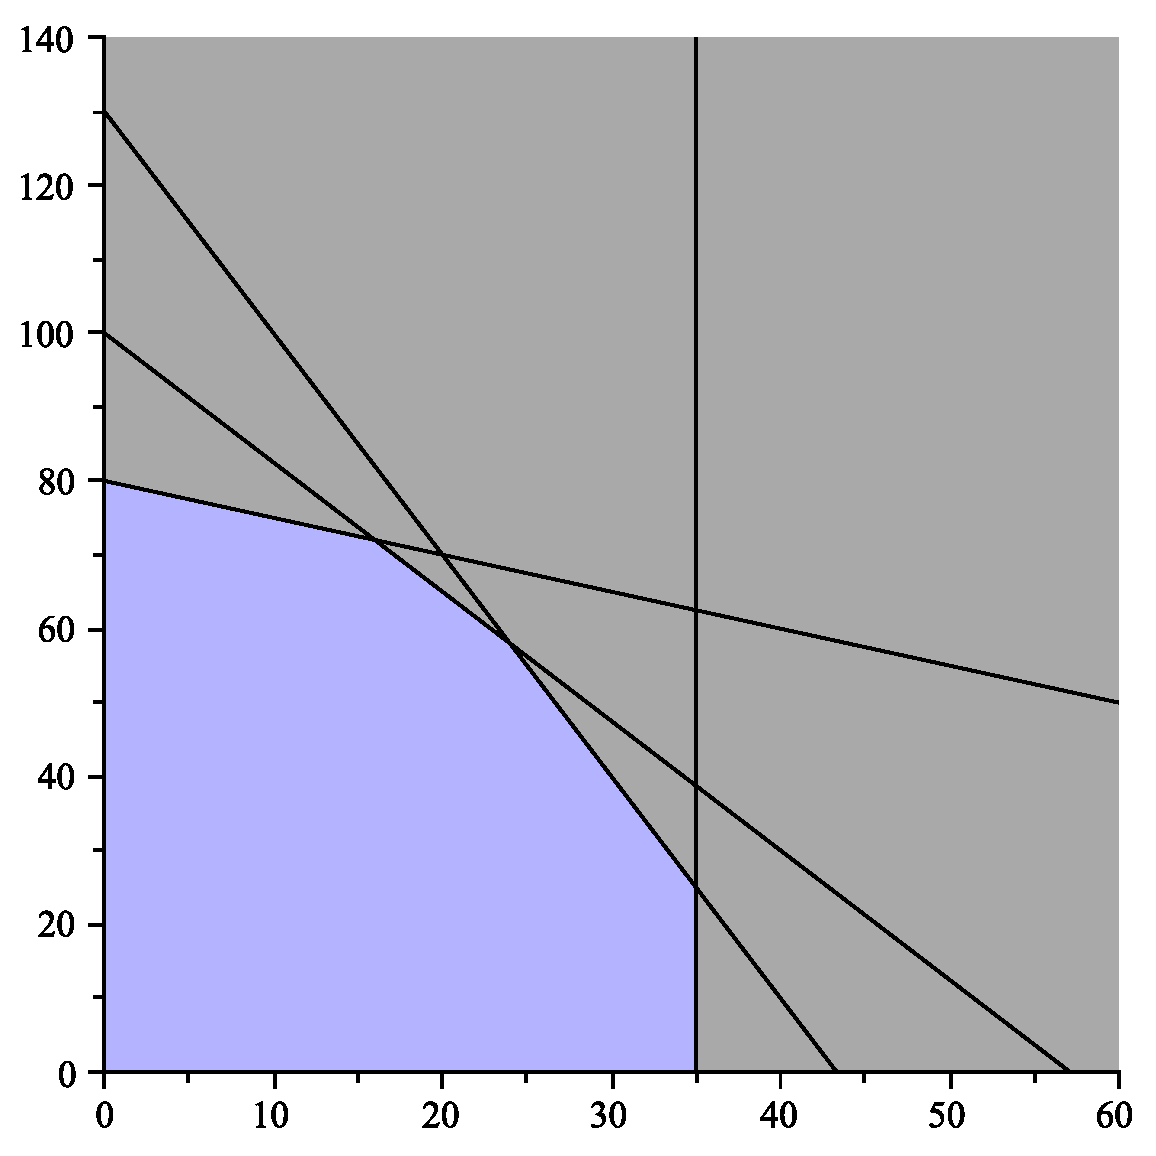
\includegraphics[scale=0.25]{DualDegeneracy3.pdf}}
\caption{Degeneracy in the primal problem causes alternative optimal solutions in the dual problem and destroys the direct relationship between the resource margin price that the dual variables represent in a non-degenerate problem.}
\label{fig:DegenDual}
\end{figure}

It should be noted that a true margin price can be computed, however this is outside the scope of the notes. The reader is referred to \cite{BJS04} (Chapter 6) for details.
\end{example}

\section{The Dual Simplex Method}
Occasionally when given a primal problem, it is easier to solve the dual problem and extract the information about the primal problem from the dual. 

\begin{example}
Consider the problem:
\begin{displaymath}
\begin{aligned}
\min\;\; & 	x_1 + 2x_2\\
s.t.\;\; &	x_1 + 2x_2 \geq 12\\
		 &	2x_1 + 3x_2 \geq 20\\
		 &	x_1, x_2 \geq 0
\end{aligned}
\end{displaymath}
To transform this problem to standard form, we would have to introduce surplus variables to obtain:
\begin{displaymath}
\begin{aligned}
\min\;\; & 	x_1 + 2x_2\\
s.t.\;\; &	x_1 + 2x_2 - s_1 = 12\\
		 &	2x_1 + 3x_2 - s_2 = 20\\
		 &	x_1, x_2, s_1, s_2 \geq 0
\end{aligned}
\end{displaymath}
In this case there is no immediately obvious initial basic feasible solution and we would have to solve a Phase I problem. Consider the dual of the original maximization problem:
\begin{displaymath}
\begin{aligned}
\max\;\;&12 w_1 + 20w_2\\
s.t.\;\; & w_1 + 2w_2 \leq 1\\
& 2w_1 + 3w_2 \leq 1\\
& w_1,w_2 \geq 0
\end{aligned}
\end{displaymath}
This is a maximization problem whose standard form is given by:
\begin{displaymath}
\begin{aligned}
\max\;\;&12 w_1 + 20w_2\\
s.t.\;\; & w_1 + 2w_2 + v_1 = 1\\
& 2w_1 + 3w_2 + v_2 = 1\\
& w_1,w_2,v_1,v_2 \geq 0
\end{aligned}
\end{displaymath}
In this case, a reasonable initial basic feasible solution for the dual problem is to set $v_1 = v_2 = 1$ and $w_1 = w_2 = 0$ (i.e., $w_1$ and $w_2$ are non-basic variables) and proceed with the simplex algorithm from this point.
\label{ex:EasyDualProblem}
\end{example}

In cases like the one illustrated in Example \ref{ex:EasyDualProblem}, we can solve the dual problem directly in the simplex tableau of the primal problem instead of forming the dual problem and solving it as a primal problem in its own tableau. The resulting algorithm is called the \textit{dual simplex algorithm}. 

For the sake of space, we will provide the dual simplex algorithm for a maximization problem:
\begin{displaymath}
P \left\{
\begin{aligned}
\max\;\;&\mathbf{c}\mathbf{x}\\
s.t.\;\;& \mathbf{A}\mathbf{x} = \mathbf{b}\\
&\mathbf{x} \geq \mathbf{0}
\end{aligned}\right.
\end{displaymath}
We will then shown how to adjust the dual simplex algorithm for minimization problems.


\begin{algorithm}
\caption{The Matrix form of the Dual Simplex Algorithm}
\label{alg:DualSimplexMatrixForm}
\begin{center}
\begin{minipage}[t]{\textwidth-1em}
\underline{\textbf{Dual Simplex Algorithm in Algebraic Form}}
\begin{enumerate*}
\item Choose an initial basic solution $\mathbf{x}_B$ and corresponding basis matrix $\mathbf{B}$ so that $\mathbf{w}\mathbf{A}_{\cdot j} - c_j \geq 0$ for all $j \in \mathcal{J}$, where $\mathcal{J}$ is the set of non-basic variables and $\mathbf{w} = \mathbf{c}_\mathbf{B}\mathbf{B}^{-1}$. 

\item Construct a simplex tableau using this initial solution.

\item If $\overline{\mathbf{b}} = \mathbf{B}^{-1}\mathbf{b} \geq \mathbf{0}$, then an optimal solution has been achieved; STOP. Otherwise, the dual problem is feasible (since $z_j - c_j \geq 0$). GOTO STEP 4.

\item Choose a \textit{leaving variable} (row) $x_{\mathbf{B}_i} = \overline{\mathbf{b}}_i$ so that $\overline{\mathbf{b}}_i < 0$.

\item Choose the index of the entering variable (column) $x_j$ ($j \in \mathcal{J}$) using the following minimum ratio test:
\begin{displaymath}
\frac{z_j - c_j}{\overline{a}_{j_i}} = \min\left\{\frac{z_k - c_k}{|\overline{a}_{k_i}|}  : k \in \mathcal{J}, \overline{a}_{k_i} < 0\right\}
\end{displaymath}

\item If no entering variable can be selected ($\overline{a}_{k_i} \geq 0$ for all $k \in \mathcal{K}$) then the dual problem is unbounded and the primal problem is infeasible. STOP.

\item Using a standard simplex pivot, pivot on element $\overline{a}_{j_i}$, thus causing $\mathbf{x}_{\mathbf{B}_i}$ to become $0$ (and thus feasible) and causing $x_j$ to enter the basis. GOTO STEP 3.
\end{enumerate*}
\end{minipage}
\end{center}
\end{algorithm}

The pivoting step works because we choose the entering variable specifically so that the reduced costs will remain positive. Just as we chose the leaving variable in the standard simplex algorithm using a minimum ratio test to ensure that $\mathbf{B}^{-1}\mathbf{b}$ remains positive, here we use it to ensure that $z_j - c_j$ remains non-negative for all $j \in \mathcal{J}$ and thus we assure dual feasibility is maintained.

The convergence of the dual simplex algorithm is outside of the scope of this course. However, it suffices to understand that we are essentially solving the dual problem in the primal simplex tableau using the simplex algorithm applied to the dual problem. Therefore under appropriate cycle prevention rules, the dual simplex does in fact converge to the optimal (primal) solution. 

\begin{theorem} In the absence of degeneracy, or when using an appropriate cycling prevention rule, the dual simplex algorithm converges and is correct.
\end{theorem}

\begin{example}
Consider the following linear programming problem:
\begin{displaymath}
\begin{aligned}
\max\;\;& -x_1 - x_2\\
s.t.\;\; &2x_1 + x_2 \geq 4\\
&x_1 + 2x_2 \geq 2\\
&x_1 , x_2 \geq 0
\end{aligned}
\end{displaymath}

Then the standard form problem is given as:
\begin{displaymath}
\begin{aligned}
\max\;\;& -x_1 - x_2\\
s.t.\;\; &2x_1 + x_2 - s_1 = 4\\
&x_1 + 2x_2 - s_2 = 2\\
&x_1, x_2 \geq 0
\end{aligned}
\end{displaymath}
The coefficient matrix for this problem is:
\begin{displaymath}
\mathbf{A} = \begin{bmatrix}
2 & 1 & -1 & 0\\
1 & 2 & 0 & -1
\end{bmatrix}
\end{displaymath}
In standard form, there is no clearly good choice for a starting basic feasible solution. However, since this is a maximization problem and we know that $x_1,x_2 \geq 0$, we know that the objective function $-x_1 - x_2$ must be bounded above by $0$. A basic solution that yields this objective function value occurs when $s_1$ and $s_2$ are both non-basic and $x_1$ and $x_2$ are both non-basic. 

If we let 
\begin{displaymath}
\mathbf{B} = \begin{bmatrix}-1 & 0\\0 & -1\end{bmatrix}
\end{displaymath}
Then we obtain the infeasible solution:
\begin{displaymath}
\overline{\mathbf{b}} = \mathbf{B}^{-1}\mathbf{b} = 
\begin{bmatrix}-4 \\ -2\end{bmatrix}
\end{displaymath}

Likewise we have:
\begin{displaymath}
\mathbf{w} = \mathbf{c}_\mathbf{B}\mathbf{B}^{-1} = \begin{bmatrix}0&0\end{bmatrix}
\end{displaymath}
since both $s_1$ and $s_2$ do not appear in the objective function. 
We can compute the reduced costs in this case to obtain:
\begin{gather*}
z_1 - c_1 = \mathbf{w}\mathbf{A}_{\cdot 1} - c_1 = 1 \geq 0\\
z_2 - c_2 = \mathbf{w}\mathbf{A}_{\cdot 2} - c_2 = 1 \geq 0\\
z_3 - c_3 = \mathbf{w}\mathbf{A}_{\cdot 3} - c_3 = 0 \geq 0\\
z_4 - c_4 = \mathbf{w}\mathbf{A}_{\cdot 4} - c_4 = 0 \geq 0\\
\end{gather*}
Thus, the fact that $\mathbf{w} \geq \mathbf{0}$ and the fact that $z_j - c_j \geq 0$ for all $j$, shows us that we have a \textit{dual feasible solution} and based on our use of a basic solution, we know that complementary slackness is ensured. 

We can now set up our initial simplex tableau for the dual simplex algorithm. This is given by:
\begin{displaymath}
\begin{array}{c}
\\
z\\
s_1\\
s_2
\end{array}
\left[
\begin{array}{c|cccc|c}
z& x_1 & x_2 & s_1 & s_2 &\text{RHS}\\
\hline
1 & 1 & 1 & 0 & 0 & 0\\
\hline
0 & -2 & -1 & 1 & 0 & -4\\
0 & -1 & \fbox{-2} & 0 & 1 & -2
\end{array}\right]
\end{displaymath}
We can choose either $s_1$ or $s_2$ as a leaving variable. For the sake of argument, suppose we choose $s_2$, the variable that's most negative as the leaving variable. Then our entering variable is chosen by comparing:
\begin{gather*}
\frac{z_1 - c_1}{|\overline{\mathbf{a}}_{21}|} = \frac{1}{|-1|}\\
\frac{z_2 - c_2}{|\overline{\mathbf{a}}_{22}|} = \frac{1}{|-2|}\\
\end{gather*}
Clearly, $1/2 < 1$ and therefore, $x_2$ is our entering variable.
\begin{displaymath}
\begin{array}{c}
\\
z\\
s_1\\
x_2
\end{array}
\left[
\begin{array}{c|cccc|c}
z& x_1 & x_2 & s_1 & s_2 &\text{RHS}\\
\hline
1 & 1/2 & 0 & 0 & 1/2 & -1\\
\hline
0 & \fbox{-3/2}	& 0 	& 1 	& -1/2 	& -3\\
0 & 1/2 	& 1 	& 0 	& -1/2 	& 1
\end{array}\right]
\end{displaymath}
At this point, we see we have maintained dual feasibility, but we still do not have primal feasibility. We can therefore choose a new leaving variable ($s_1$) corresponding to the negative element in the RHS. The minimum ratio test shows that this time $x_1$ will enter and the final simplex tableau will be:
\begin{displaymath}
\begin{array}{c}
\\
z\\
x_1\\
x_2
\end{array}
\left[
\begin{array}{c|cccc|c}
z& x_1 & x_2 & s_1 & s_2 &\text{RHS}\\
\hline
1 & 0 & 0 & 1/3 & 1/3 & -2\\
\hline
0 & 1		& 0 	& -2/3 	& 1/3 	& 2\\
0 & 0 		& 1 	& 1/3 	& -2/3 	& 0
\end{array}\right]
\end{displaymath}
It's clear this is the optimal solution to the problem since we've achieved primal and dual feasibility and complementary slackness. It's also worth noting that this optimal solution is degenerate, since there is a zero in the right hand side. 
\end{example}

\begin{exercise} Prove that the minimum ratio test given in the dual simplex algorithm will maintain dual feasibility from one iteration of the simplex tableau to the next. [Hint: Prove that the reduced costs remain greater than or equal to zero, just as we proved that $\overline{\mathbf{b}}$ remains positive for the standard simplex algorithm.]
\end{exercise}